
\begin{frame}
\begin{figure}

\vspace{-1cm}	
\hspace{-4cm}		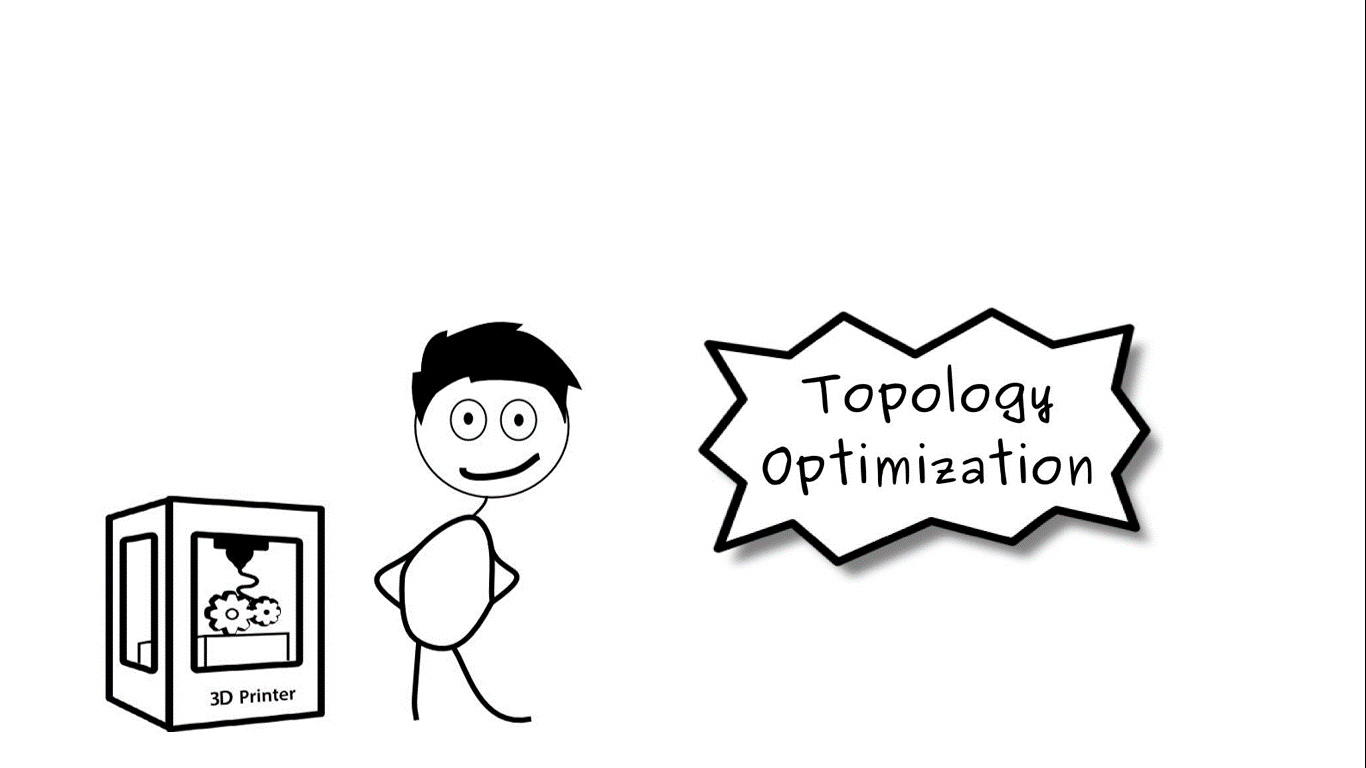
\includegraphics[width=1\linewidth]{Pictures/animations/animation_1.png}
		\end{figure}

\end{frame}

\begin{frame}
\begin{figure}
			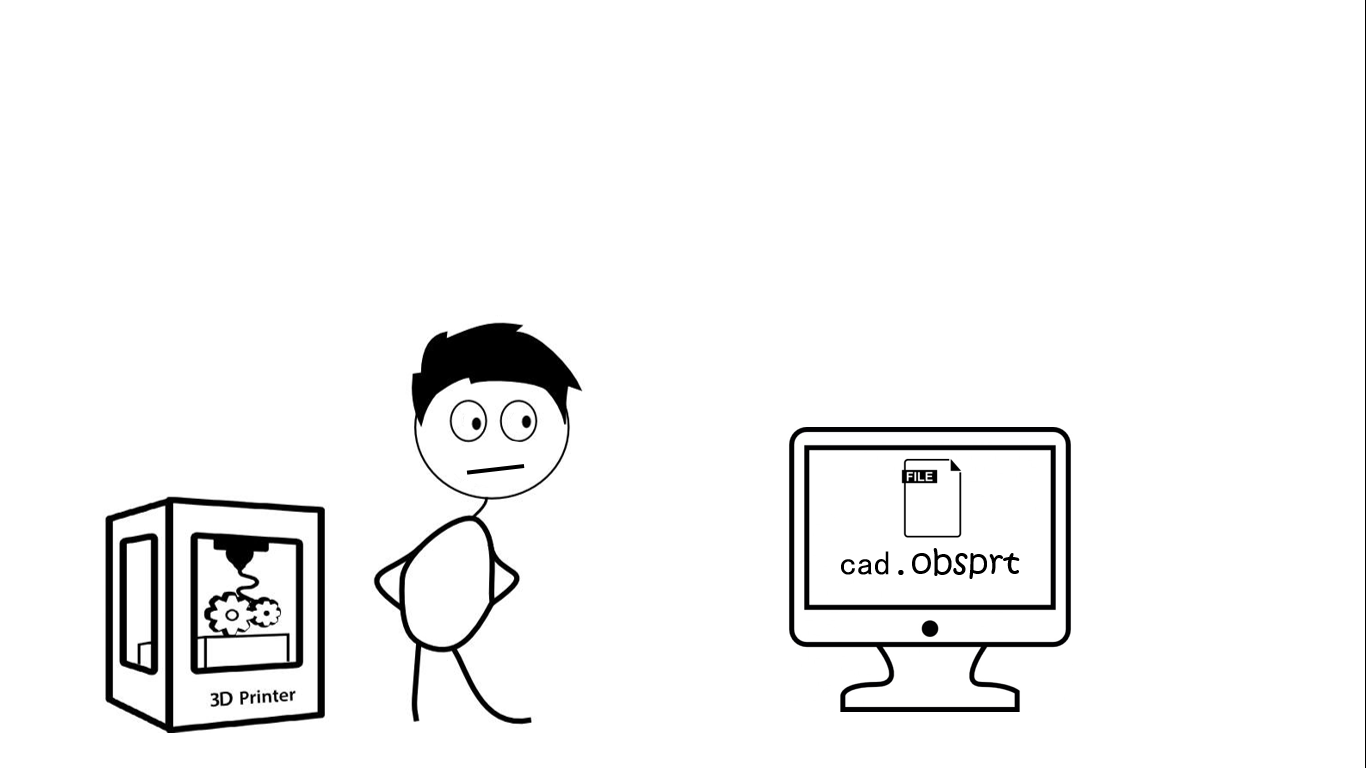
\includegraphics[width=1.4\linewidth]{Pictures/animations/animation_2.png}
		\end{figure}

\end{frame}

\begin{frame}{How hard is it to design a lamp?}

	\begin{multicols}{2}
		%\underline{Problem:}
		\setbeamercolor{block}{bg=white,fg=cyan}
		\begin{block}{Problem:}{
		\begin{itemize}		
			\item The Engineer designer pendulum			
		\end{itemize}~\\
		}
		%\begin{variableblock}{Focus:}{bg=cyan,fg=white}	
		\end{block}
	
		\vfill
		\columnbreak


		\begin{block}{Desired:}{
		\begin{itemize}		
			\item[$\Rightarrow$] One click optimization				
		\end{itemize}~\\
		}
		\end{block}
				
		\end{multicols}
		\pause
		
	\begin{multicols}{2}

		\begin{itemize}
			\item Top-Opt algorithms are a one way street
		\end{itemize}~\\
		\vfill
		\columnbreak
		\begin{itemize}
			\item[$\Rightarrow$] A full circle optimization process	
		\end{itemize}~\\			
		\end{multicols}
		\pause
	\begin{multicols}{2}

		\begin{itemize}
			\item Exotic input file types
		\end{itemize}~\\
		\vfill
		\columnbreak
		\begin{itemize}
			\item[$\Rightarrow$] Standardized input files	
		\end{itemize}~\\			
		\end{multicols}

\end{frame}	

\begin{frame}{What they get}	
\begin{itemize}
			\item One-step solution process	
			\item Full 3-D optimization via Finite Elements
			\item Production-ready output geometry
			\end{itemize}~\\
\end{frame}	

\begin{frame}{DEMO}

\end{frame}

\begin{frame}{Features}

\begin{block}{Fully integrated design process}{
		\begin{itemize}		
			\item CAD to CAD
			\item Turnkey
			\item Standardized I/O			
		\end{itemize}~\\
		}
		\end{block}
\pause
\begin{block}{Control to the user}{
		\begin{itemize}		
			\item Resolution
			\item Smoothness
			\item Localized Optimization			
		\end{itemize}~\\
		}
		\end{block}
\pause		
\begin{block}{100\% open source}{
		%\begin{itemize}		
		%\end{itemize}~\\
		}
		\end{block}

\end{frame}
		